\documentclass[10pt, handout]{beamer}

%\usepackage[backend=bibtex,firstinits=true,style=verbose-inote,citestyle=authortitle]{biblatex}
\usepackage{bm}
\usepackage{subcaption}
\usepackage{graphicx}
\usepackage{subcaption}
\usepackage{amsmath}
\usepackage{amsfonts}
\usepackage{dsfont}
\usepackage{makecell}
% \usepackage{filecontents}
\usepackage{biblatex}
% \newcommand{\expect}[2][]{
\ifthenelse{\equal{#1}{}}{
\mathbb{E}\left[#2\right]
}{
\underset{#1}{\mathbb{E}}\left[#2\right]
}}

\newcommand{\cov}[2][]{
\ifthenelse{\equal{#1}{}}{
\text{Cov}\left[#2\right]
}{
\underset{#1}{\text{Cov}}\left[#2\right]
}}


\newcommand{\var}[2][]{
\ifthenelse{\equal{#1}{}}{
\text{Var}[#2]
}{
\underset{#1}{\text{Var}}[#2]
}}

\newcommand{\loss}[2][]{
\ifthenelse{\equal{#1}{}}{
\mathcal{L}(#2)
}{
\mathcal{L}_{#1}(#2)
}}

\newcommand{\kl}[2]{
\text{D}_\text{KL}[#1 \parallel #2]
}

\newcommand{\R}{\mathbb{R}}
%\newcommand{\Prob}{\mathbb{P}}

\newcommand{\1}[1]{\mathds{1}\{#1\}}


%\usecolortheme{dolphin}
\setbeamertemplate{navigation symbols}{}
\setbeamertemplate{section in toc}{\inserttocsectionnumber.~\inserttocsection}


\addbibresource{references.bib}


\title{Model Compression}
%\subtitle{}
\author{Ivan Skorokhodov}
%\date{}
%\logo{
\includegraphics[height=1cm]{images/ipavlov-logo.png}}

\newcommand{\citepaper}[1]{\citetitle{#1} by \citeauthor{#1}}

%\graphicspath{{./images}}

%\usetheme{lucid}
\begin{document}

\begin{frame}
    \titlepage
\end{frame}

\begin{frame}{Overview}
    \tableofcontents
\end{frame}

% \section{Motivation}
% \begin{frame}
%     \begin{itemize}
%         \pause\item Accelerating inference or training
%         \pause\item Reducing memory footprint
%         \pause\item Theoretical curiosity
%     \end{itemize}
% \end{frame}

\section{Pruning}
\begin{frame}
    Pruning
\end{frame}

\begin{frame}{Pruning}
    \begin{itemize}
        \pause\item \textit{Pruning} is removing weights/neurons in a model while preserving the accuracy
        \pause\item It can be done at different stages:
        \begin{itemize}
            \pause\item before training (\textit{foresight pruning})
            \pause\item during training
            \pause\item after training
            \pause\item iteratively train/prune several times
        \end{itemize}
    \end{itemize}
\end{frame}


\subsection{Pruning weights}
\begin{frame}{Pruning weights}
\begin{itemize}
    \pause\item Simplest strategies:
    \begin{itemize}
        \pause\item Apply $L_1$-regularization during training
        \pause\item Prune based on weights magnitudes after training
        \pause\item Iterative Magnitude Pruning (IMP): ``train $\to$ prune by magnitude $\to$ restore original init'' several times
    \end{itemize}
    \pause\item Variational dropout:
    \begin{itemize}
        \pause\item Perform a variational inference for model weights
        \pause\item Obtain $\mu_i, \sigma_i^2$ associated with each weight
        \pause\item If $\sigma_i^2$ is large, then the weight is not important $\Rightarrow$ prune it
    \end{itemize}
    \pause\item Single-Shot Network Pruning (SNIP) prunes at initialization \cite{SNIP}:
    \begin{itemize}
        \pause\item Compute how much a weight influences the loss:
        \begin{equation}
S\left(\theta_{i}\right)=\lim _{\epsilon \rightarrow 0}\left|\frac{\mathcal{L}\left(\theta_{i}\right)-\mathcal{L}\left(\theta_{i}+\epsilon \right)}{\epsilon}\right|=\left|\frac{\partial \mathcal{L}}{\partial \theta_{i}}\right|
\end{equation}
        \pause\item Prune weights with low scores
    \end{itemize}
\end{itemize}
\end{frame}


\begin{frame}{Lottery Ticket Hypothesis (LTH)}
\pause
LTH \cite{LTH}: \textit{A neural network contains a subnetwork (winning ticket) which, when being trained in isolation, achieves the same accuracy as the base model and does so in the same number of iterations or even faster.}

\medskip
\pause

One finds a winning ticket with Iterative Magnitude Pruning (IMP) in $n$ iterations:
\begin{enumerate}
    \pause\item Randomly initialize a neural network $f_{\theta_0}$, initialize a mask $m^{(0)}$ of all-ones.
    \pause\item Train for $T$ iterations, obtain $\theta_T$.
    \pause\item Remove $p^{1/n}$ percent of the lowest-magnitude parameters from $\theta_T$ by updating the mask $m^{(\ell)}$.
    \pause\item Reset the remaining parameters to $\theta_0 \odot m^{(\ell)}$.\footnote{\cite{Stabilizing_LTH} found out that it is more beneficial to \textit{rewind} the weights to some $\theta_k$ with $k \ll T$ instead of resetting them to $\theta_0$}
    \pause\item Repeat steps 2-4 $n$ times, obtain the winning ticket $\theta_0 \odot m^{(n)}$.
\end{enumerate}
\end{frame}


\begin{frame}{LTH: caveats}
\begin{itemize}
    \pause\item \cite{State_of_sparsity, Rethinking_Pruning} showed that LTH idea works poorly for large datasets
    \pause\item IMP requires several full training procedures to work well
    \begin{figure}
        \centering
        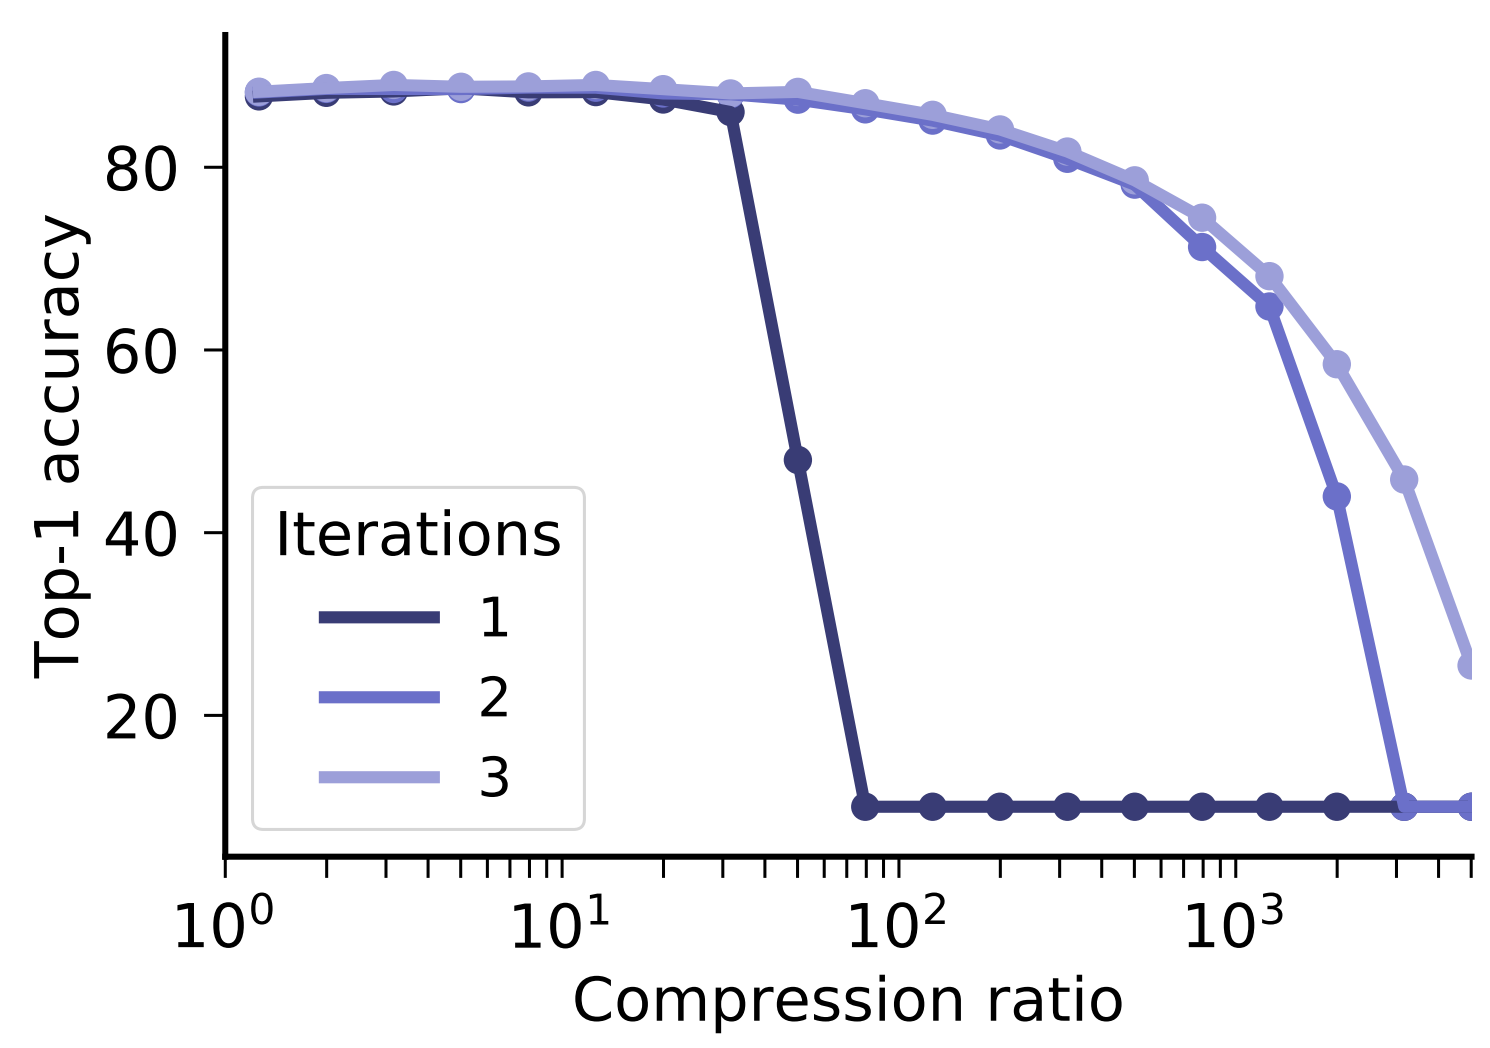
\includegraphics[width=0.5\textwidth]{images/imp-num-iters.png}
        %\caption{Caption}
        \label{fig:imp-num-iters}
    \end{figure}
    \pause\item This motivates \textit{foresight pruning}: removing weights once and without training \cite{SNIP, GraSP, SynFlow}
\end{itemize}
\end{frame}


\begin{frame}{Synaptic saliency}
\begin{itemize}
    \pause\item All pruning algorithms remove weights based on score values $S(\theta_i)$ associated with each weight $\theta_i$
    \pause\item These scores can often be represented as
\begin{equation}\label{eq:syn-saliency}
    S(\theta)=\frac{\partial R}{\partial \theta} \odot \theta
\end{equation}
for a function $R(\theta)$ which \textit{operates on top of model outputs $f_\theta(x)$}
    \pause\item If a score function can be represented as \eqref{eq:syn-saliency} then it is called \textit{synaptic saliency} \cite{SynFlow}
    \pause\item Intuitively, it represents weight importances (but in general can be negative)
\end{itemize}
\end{frame}


\begin{frame}{Synaptic saliency in real life}
\pause Many pruning algorithms have a form similar to \eqref{eq:syn-saliency}:
\begin{itemize}
    \pause\item Skeletonization \cite{Skeletonization}:
    \begin{equation}
        \mathcal{R}(\theta) = -L(\theta) \Longrightarrow S(\theta)= -\frac{\partial \mathcal{L}}{\partial \theta} \odot \theta
    \end{equation}
    
    \pause\item SNIP \cite{SNIP} has a similar form:
    \begin{equation}
        S(\theta) = \left| \frac{\partial \mathcal{L}}{\partial \theta} \odot \theta \right|
    \end{equation}
    
    \pause\item GraSP \cite{GraSP} has a similar form:
    \begin{equation}
        S(\theta) = \left(- \mathcal{H}\frac{\partial \mathcal{L}}{\partial \theta} \right) \odot \theta
    \end{equation}
    
    \pause\item Magnitude Pruning is not a synaptic saliency:
    \begin{equation}
        S(\theta_i) = \theta_i^2 = \frac{\partial \mathcal{R}(\theta)}{\partial \theta} \odot\theta \quad\text{for}\quad \mathcal{R}(\theta) = \frac{1}{2}\| \theta \|_2^2,
    \end{equation}
    but $\mathcal{R}(\theta)$ is not a function of outputs!
\end{itemize}
\end{frame}


\begin{frame}{Neuron saliency}
\pause
Synaptic saliency gives rise to \textit{input/output neuron saliency}.
\pause
Let:
\begin{itemize}
    \item $\Omega^\text{in}(\nu)$ be the set of incoming weights for neuron $\nu$
    \item $\Omega^\text{out}(\nu)$ be the set of outcoming weights for neuron $\nu$
\end{itemize}

\pause
Then:
\begin{equation}
    S^\text{in}_\nu = \sum_{\theta_i \in \Omega^\text{in}(\nu)} S(\theta_i)
    \quad\text{and}\quad
    S^\text{out}_\nu = \sum_{\theta_i \in \Omega^\text{out}(\nu)} S(\theta_i)
\end{equation}
\begin{figure}
    \centering
    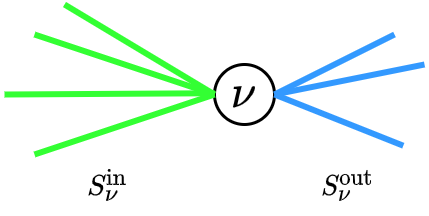
\includegraphics[width=0.3\textwidth]{images/neuron-saliency.png}
    \caption{Neuron saliency}
    \label{fig:neuron-saliency}
\end{figure}
\end{frame}

\begin{frame}{Layer saliency}
\pause
Neuron saliency gives rise to a \textit{layer saliency}.
Let $x^\ell$ be a vector of neurons in layer $\ell$, then layer saliency $S^\ell$ is:

\begin{equation}
    S^\ell = \sum_{i} S_{x^\ell_i}^\text{in}
\end{equation}

\pause
One can show that for a homogenous activation function $\phi$ we have\footnote{$\phi(x) = x \cdot \phi'(x)$ --- holds for ReLU, LeakyReLU, linear}:
\begin{align}
    S^\text{in}_\nu = \frac{\partial R}{\partial x_\nu} x_\nu
    \quad\text{and}\quad
    S^\text{out}_\nu = \frac{\partial R}{\partial \phi(x_\nu)} \phi(x_\nu),
\end{align}
where $x_\nu$ is a neuron's value before the non-linearity.
\pause
This gives us:
\begin{equation}
    S^\ell = \left\langle \frac{\partial R}{\partial x^\ell}, x^\ell \right\rangle
\end{equation}
\end{frame}

\begin{frame}{Conservation laws}
Authors proved two conservation laws.
If a model's activations are homogenous, then:
    \begin{enumerate}
        \pause\item (Neuron-wise conservation) $S_\nu^\text{in} = S_\nu^\text{out}$ for all neurons $\nu$
        \pause\item (Network-wise conservation) $S^{\ell} = S^{\ell'}$ for all layers $\ell, \ell'$
    \end{enumerate}
\end{frame}


\begin{frame}{Conservation laws in practice}
    Authors measured how the conservation holds in practice:
    \begin{figure}
        \centering
        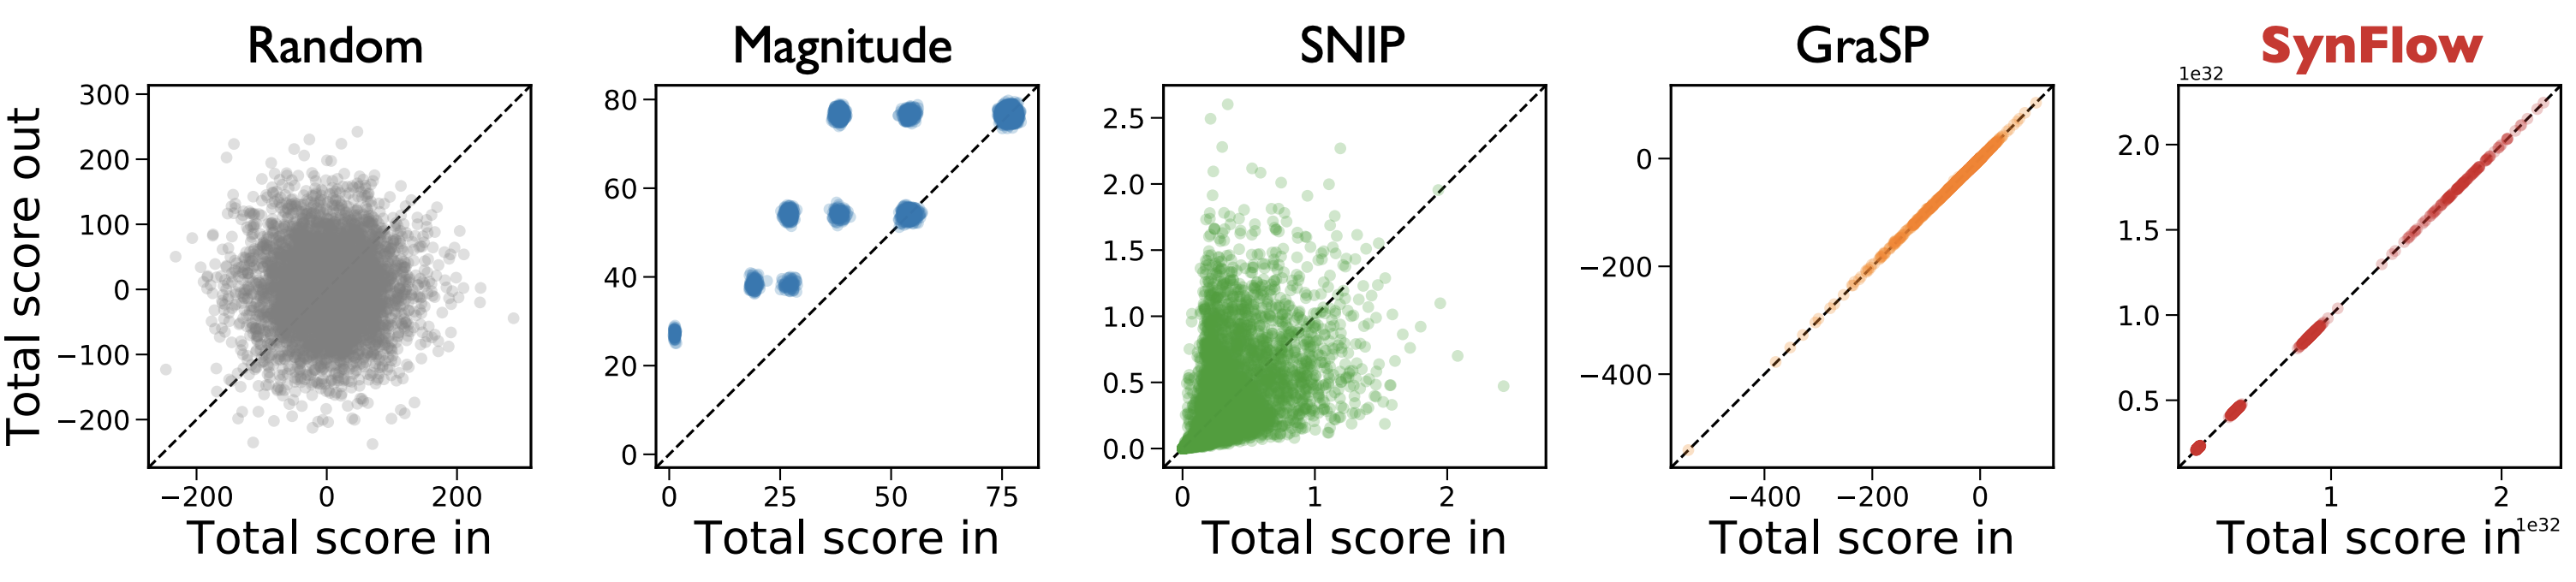
\includegraphics[width=\textwidth]{images/neuron-wise-conservation.png}
        \caption{Input/output score values for each neuron at initialization for VGG-19 model on ImageNet}
        \label{fig:neuron-wise-conservation}
    \end{figure}
\end{frame}


\begin{frame}{Layer collapse}

\begin{figure}
    \centering
    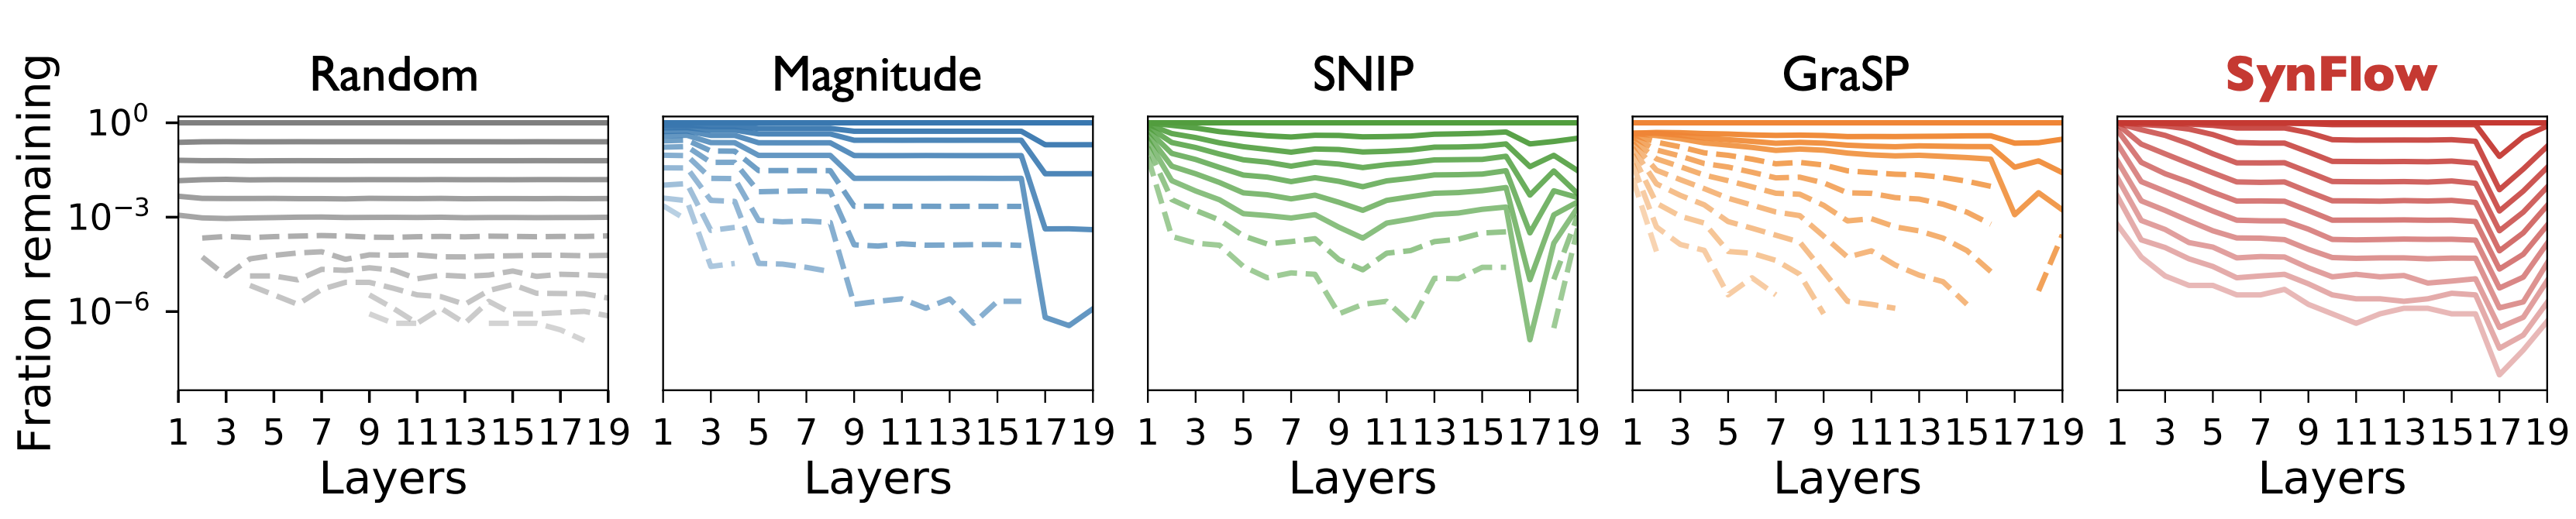
\includegraphics[width=\textwidth]{images/layer-collapse.png}
    \caption{Fraction of weights remaining in each layer for VGG-19 at initialization on ImageNet. Dashed lines indicates that there is at least one layer without any parameters at all.}
    \label{fig:layer-collapse}
\end{figure}
\begin{itemize}
    \item Many pruning algorithms suffer from layer collapse: they prune all the weights in a single layer
    \pause\item In practice, large layers become over-pruned
    \pause\item Network-wise conservation law explains this:
    \begin{itemize}
        \pause\item since $S^\ell = S^{\ell'}$ for all layers, then parameters in a large layer on average have much smaller scores
    \end{itemize}
\end{itemize}
\end{frame}


\begin{frame}{Alleviating layer collapse}
    \begin{itemize}
        \pause\item To formalize layer-collapse, authors state the ``Maximal Critical Compression Axiom'': \textit{a pruning algorithm is good, if it does not prune all the parameters in a single layer if there is something left to prune in other layers}
        \pause\item One way to avoid layer collapse is local masking: prune each layer individually, but this performs far worse \cite{SynFlow}
        \pause\item Instead authors provide the following solution
    \end{itemize}
    \textbf{Theorem}. \textit{If a pruning algorithm, with global-masking, assigns positive scores that respect layer-wise conservation and if the algorithm re-evaluates the scores every time a parameter is pruned, then the algorithm satisfies the Maximal Critical Compression axiom.}
\end{frame}


\begin{frame}{Synaptic Flow}
    \pause
    Following the theorem's idea they propose \textit{Synaptic Flow (SynFlow)} pruning algorithm:
    \begin{equation}\label{eq:synflow-r-function}
\mathcal{R}_{\mathrm{SF}}=\mathds{1}^{T}\left(\prod_{\ell=1}^{L}\left|\theta^{[\ell]}\right|\right) \mathds{1}
\end{equation}
    
\pause
One can show that:
\begin{equation}\label{eq:synflow-score-function}
\mathcal{S}_{\mathrm{SF}}\left(w_{i j}^{[\ell]}\right)
=
\underbrace{\left[\mathds{1}^{\top} \prod_{k=\ell+1}^{N}\left|W^{[k]}\right|\right]_{i}}_{\text{further connections importance}}
\cdot
\left|w_{i j}^{[\ell]}\right|
\cdot
\underbrace{\left[\prod_{k=1}^{\ell-1}\left|W^{[k]}\right| \mathds{1}\right]_{j}}_{\text{previous connections importance}}
\end{equation}

\pause
\begin{itemize}
    \item\pause It is an iterative algorithm, applied $n=100$ times in practice (at initialization)
    \item\pause The magic is that it does not use any data!
\end{itemize}
\end{frame}

\begin{frame}{SynFlow results}
    \begin{figure}
        \centering
        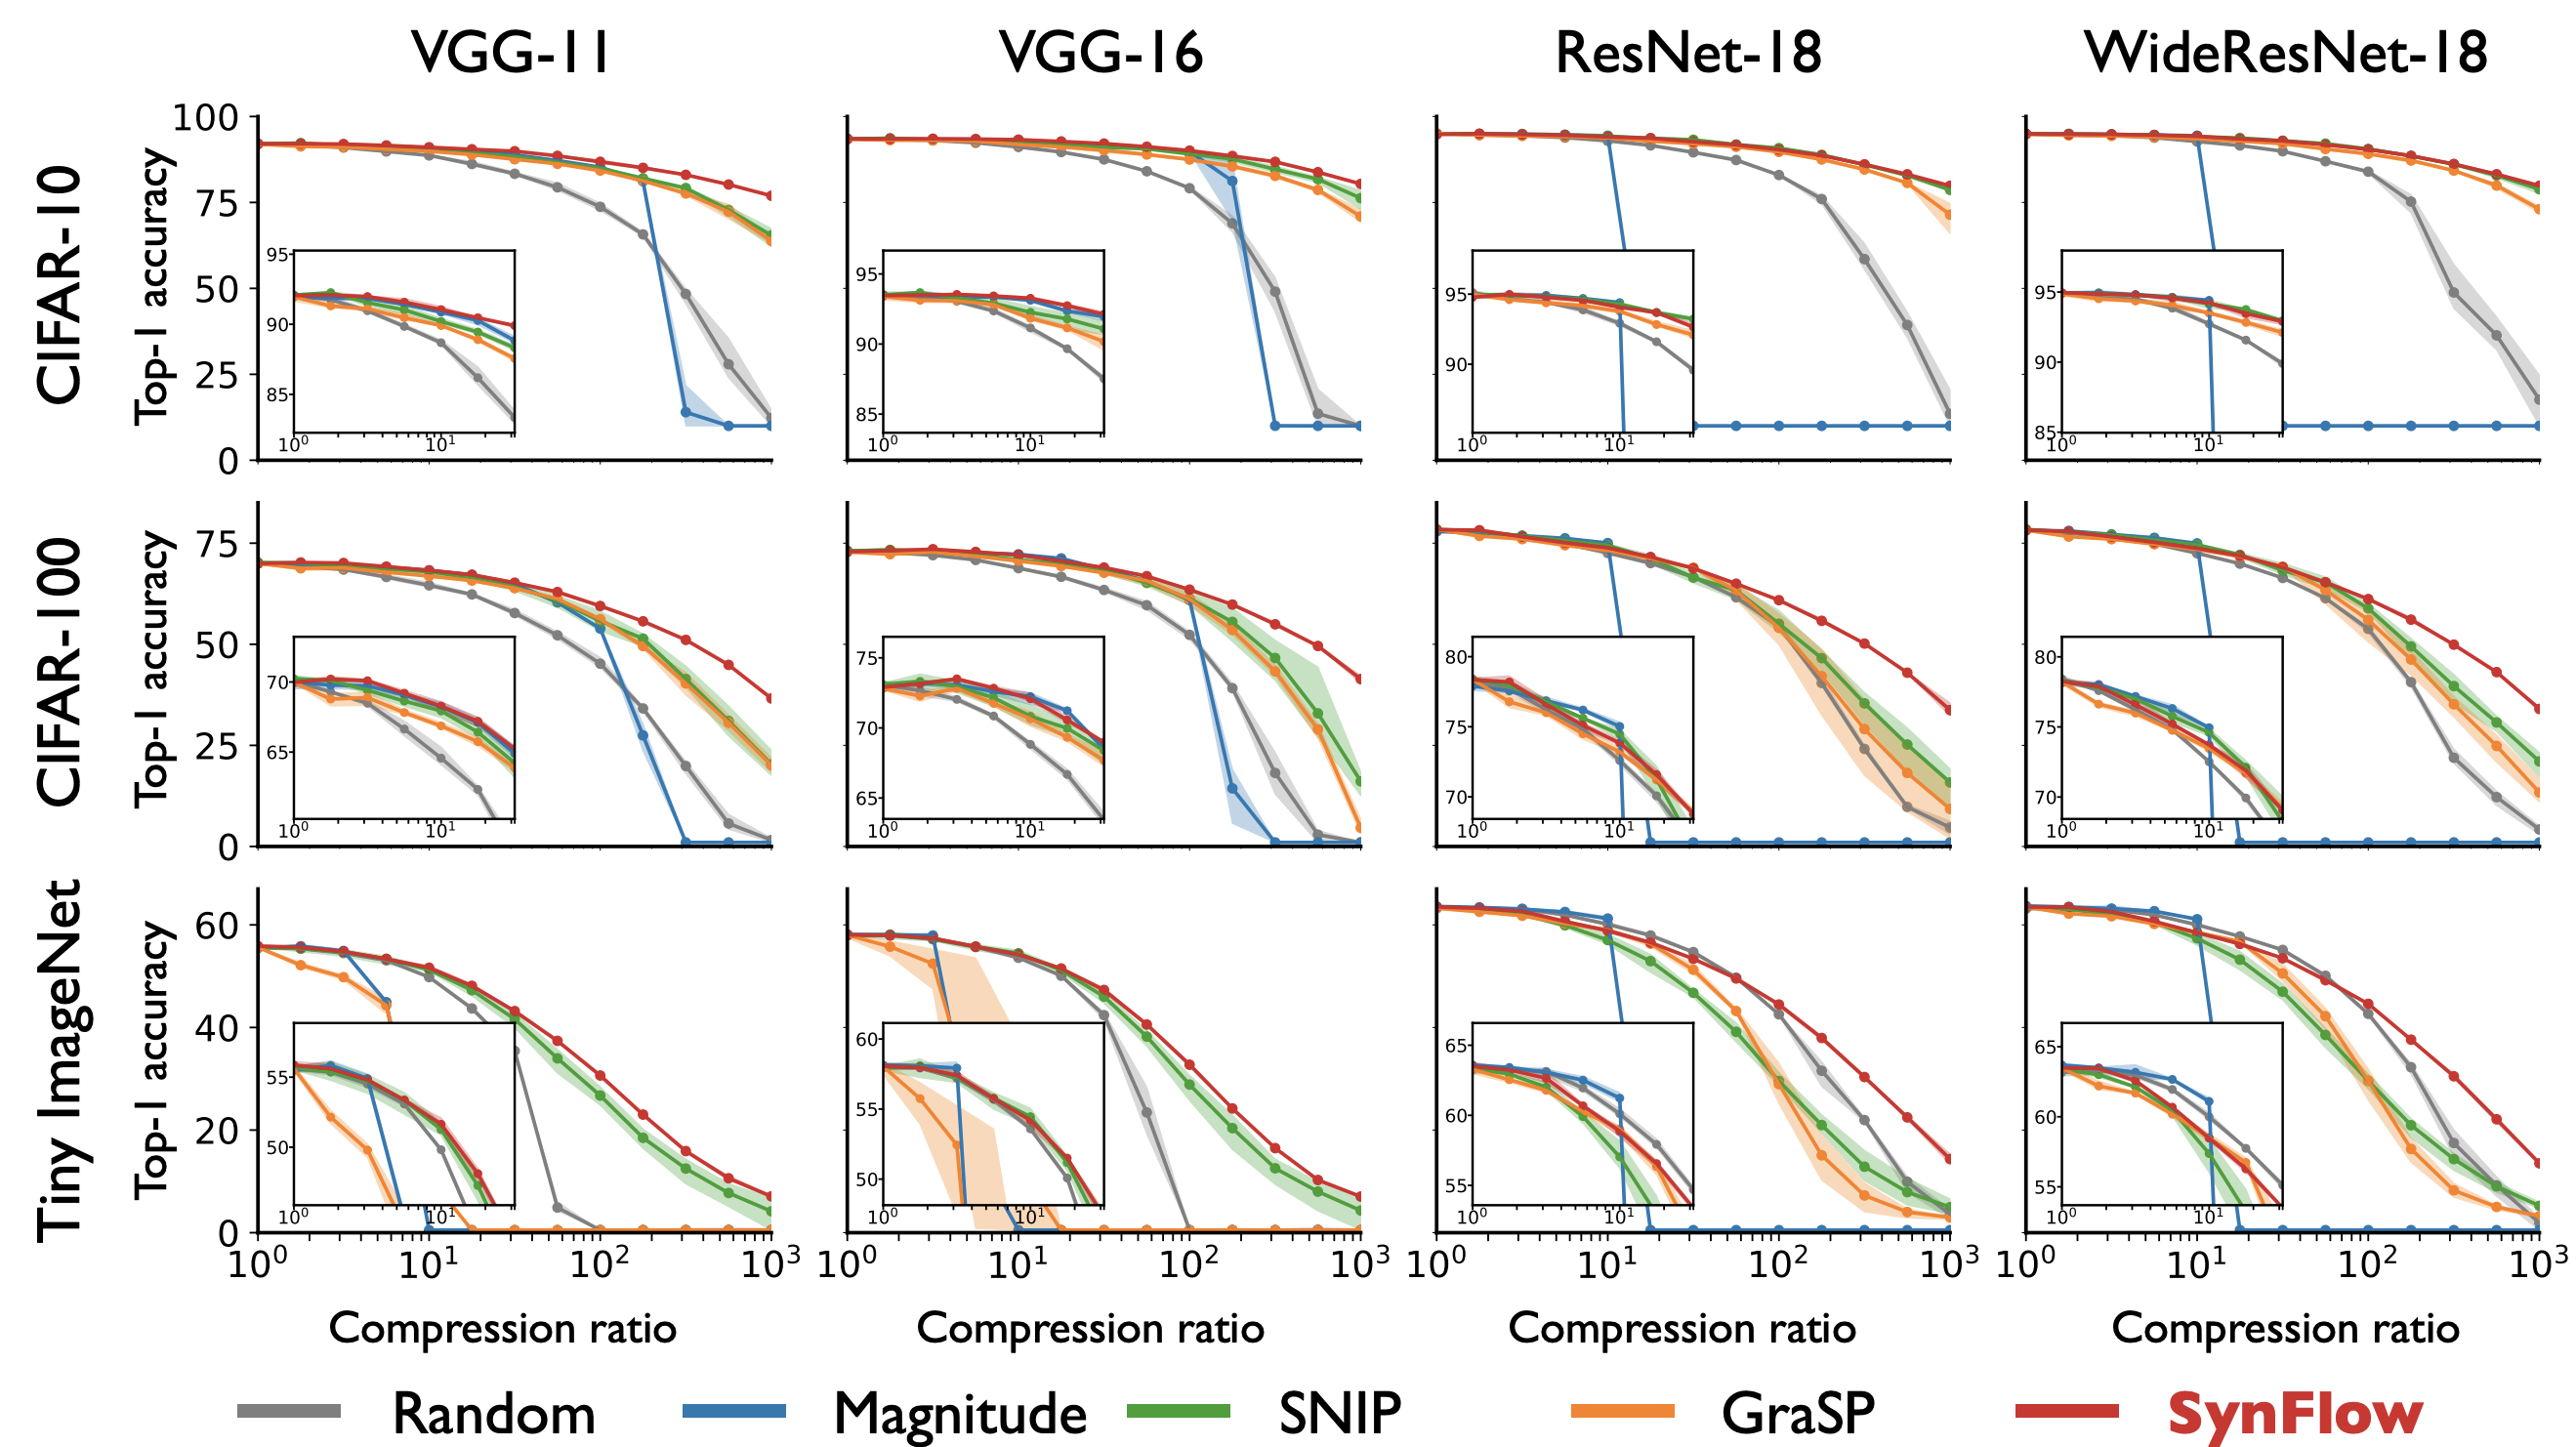
\includegraphics[width=\textwidth]{images/synflow-results.png}
        % \caption{SynFlow results for VGG-16 on CIFAR-100}
        % \label{fig:synflow-results}
    \end{figure}
\end{frame}


\begin{frame}{A problem with SynFlow}
    \begin{itemize}
        \pause\item $\mathcal{R}_\text{SF}(\theta)$ is not a function of the outputs (but ``close'': it is a function of the outputs of a model with all weights replaced with their absolute values).
        \pause\item If we'll now generalize synaptic saliency definition to encompass such functions, then magnitude pruning would also be a positive synaptic saliency
        \pause\item Then it would have to satisfy a theorem that it does not lead to layer collapse when applied iteratively (but it does)
    \end{itemize}
\end{frame}

% \begin{frame}{Conclusion}
% \pause
% Strong points
% \begin{itemize}
%     \pause\item An interesting ``physical'' theory on signal propagation
%     \pause\item Data-free foresight pruning
% \end{itemize}

% \pause
% Weak points
% \begin{itemize}
%     \pause\item 123
%     \pause\item Authors do not test on ImageNet
% \end{itemize}
% \end{frame}


\subsection{Pruning neurons}
\begin{frame}{Pruning neurons (\textit{structured pruning})}

\pause
Pruning neurons is usually based on weights pruning:
\begin{itemize}
    \pause\item Magnitude pruning: prune neurons which weights have the lowest magnitude
    \pause\item Vardrop pruning: prune neurons which weights have the highest variance
\end{itemize}

\pause
It is usually required to fine-tune the model afterwards.
\end{frame}

% \begin{frame}{Structured Sparsity Learning}
%     Structured Sparsity Learning (SSL) \cite{SSL} prunes weights in groups
% \end{frame}

\begin{frame}{Network slimming}
\begin{itemize}
    \pause\item Network Slimming \cite{Network_slimming} associates a scaling parameter $\gamma_{\ell, k}$ for channel $k$ in layer $\ell$ and regularizes them during training:
    \begin{equation}
        \mathcal{L}(\theta, \gamma) = \mathcal{L}_\text{data}(\theta, \gamma) + \lambda \sum_{\ell, k} \| \gamma_{\ell, k} \|
    \end{equation}
    \pause\item After training it is necessary to fine-tune the pruned model
    \pause\item These scalings can be merged with BatchNorm
\end{itemize}

\pause
\begin{figure}
    \centering
    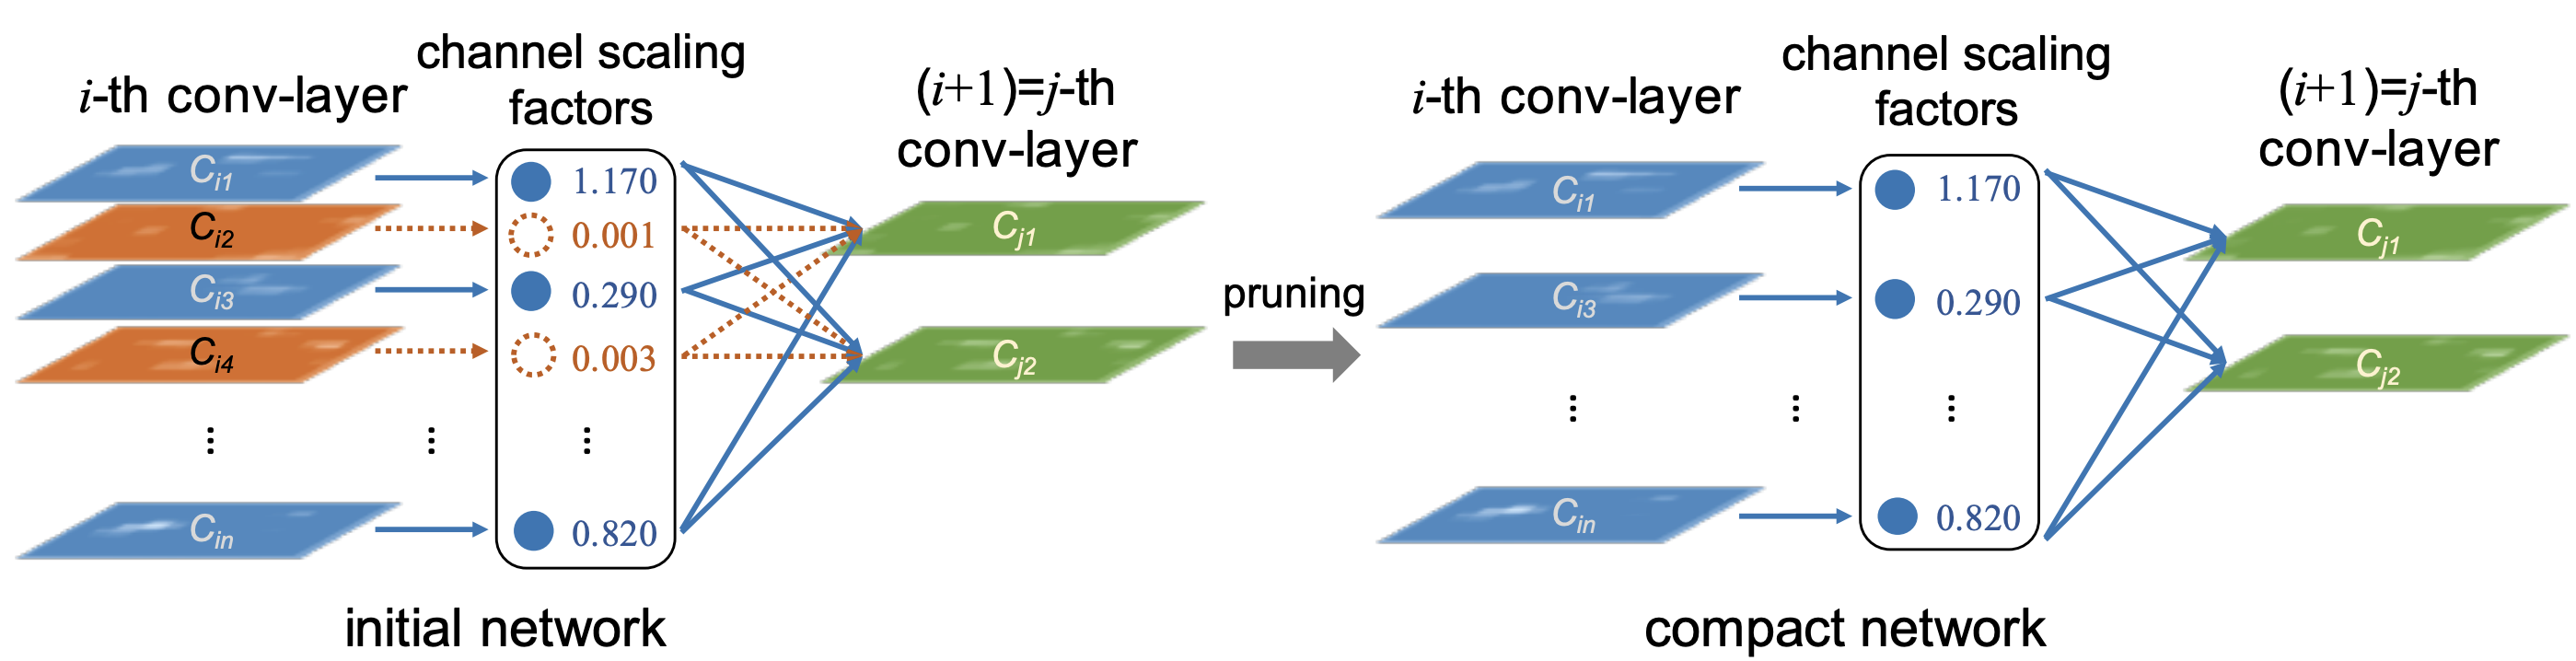
\includegraphics[width=\textwidth]{images/network-slimming.png}
\end{figure}
\end{frame}

\begin{frame}{Network Slimming results}
\begin{figure}
    \centering
    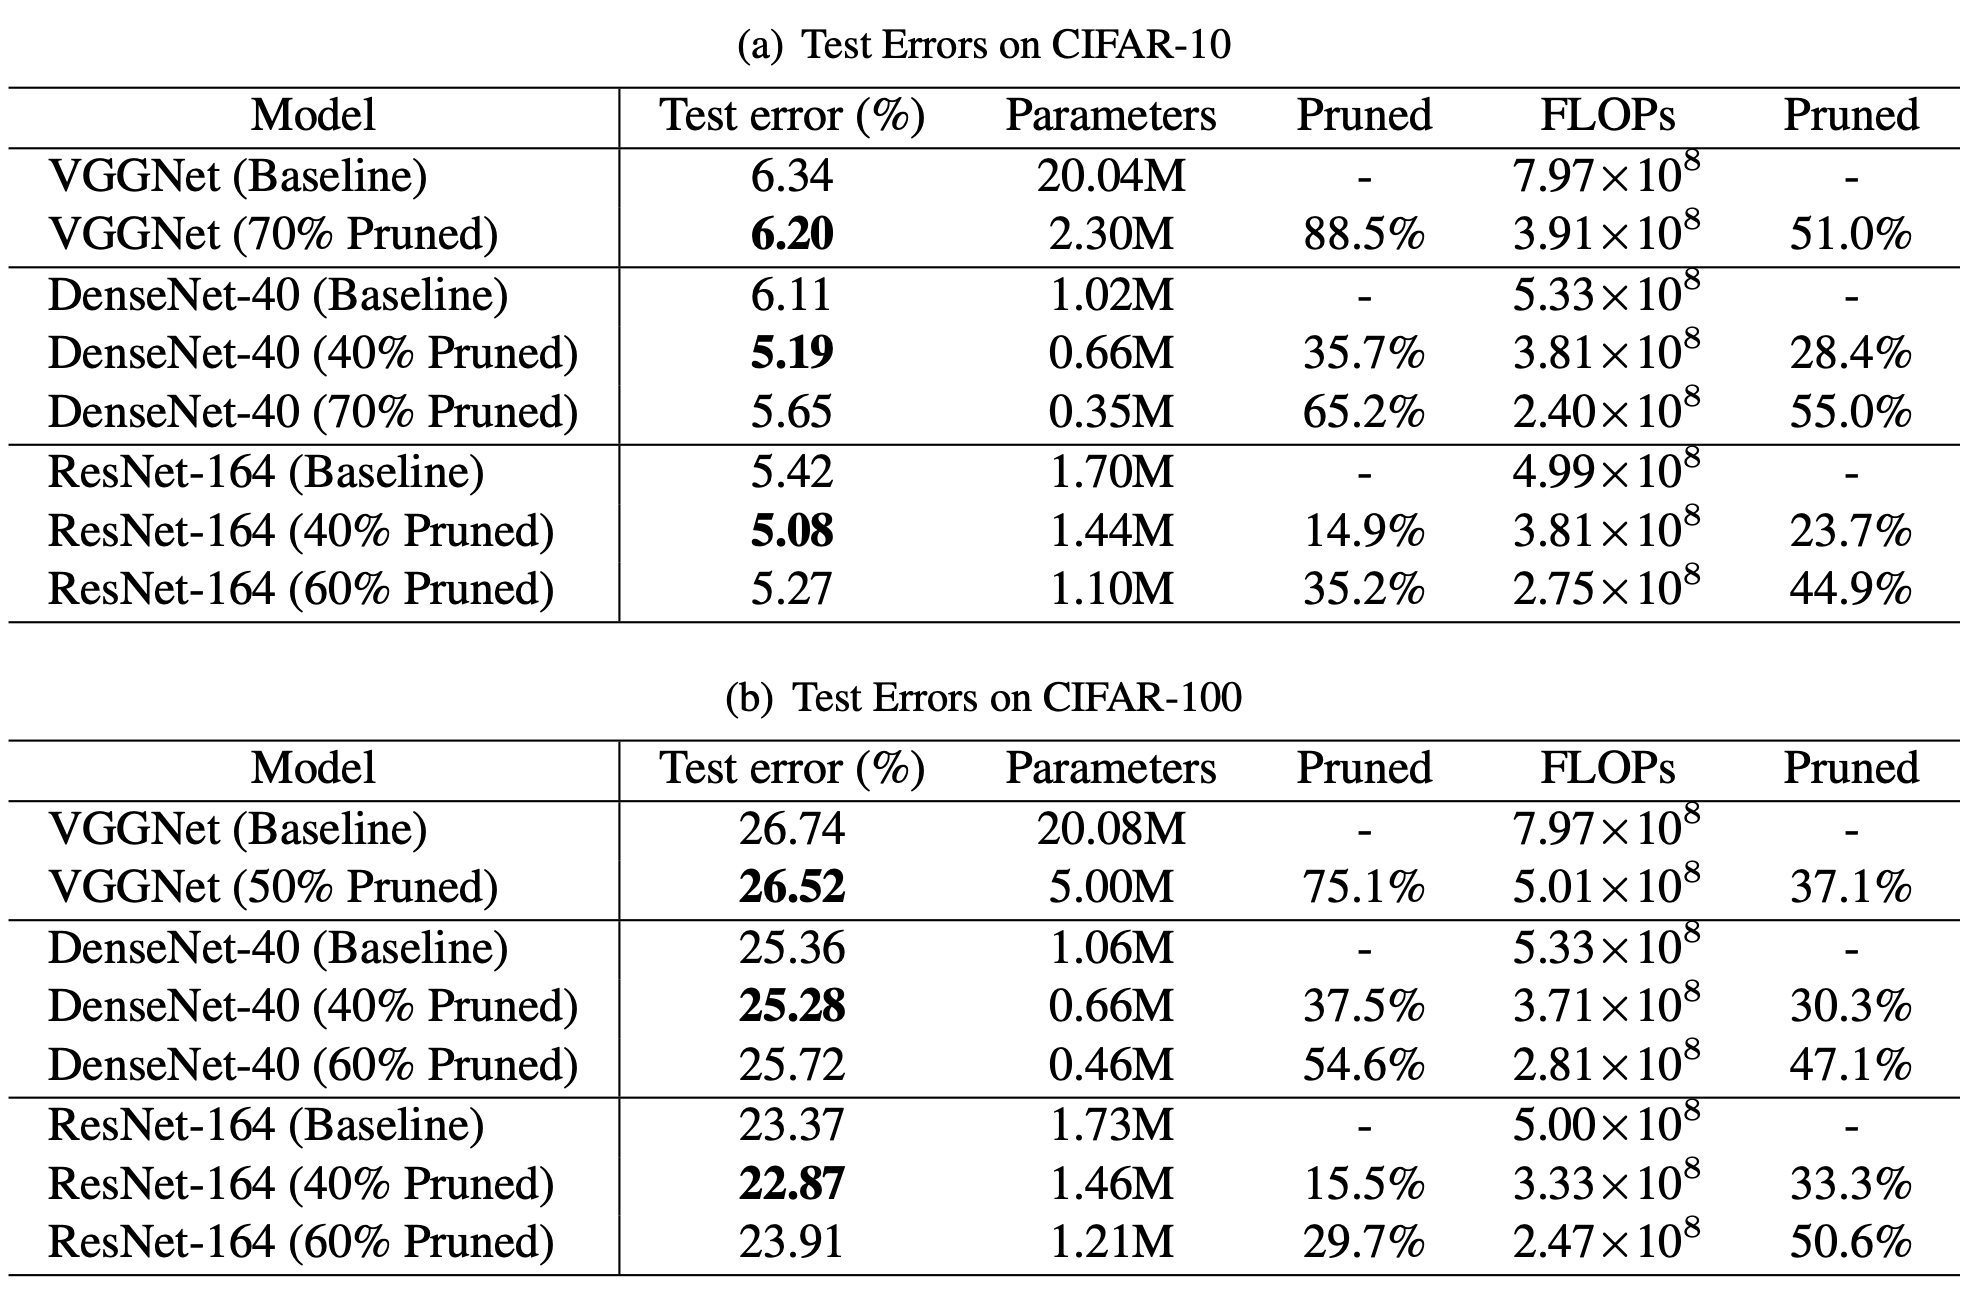
\includegraphics[width=0.8\textwidth]{images/network-slimming-results.png}
    \caption{Pruning can also have a regularization effect: pruned models perform better}
\end{figure}
\end{frame}

\begin{frame}{Pruning caveats}
\begin{itemize}
    \pause\item Pruning weights (theoretically) reduces the number of FLOPs, but:
    \begin{itemize}
        \pause\item Resulted sparse matrices are not ``sparse enough'' to provide practical benefits (sparse matrix-vector multiplications are usually based on non-parallel computations)
        \pause\item \cite{State_of_sparsity, Rethinking_Pruning} claim that modern SotA weight-pruning algorithms work poorly on large datasets
    \end{itemize}
    \pause\item Pruning neurons speeds up a model, but:
    \begin{itemize}
        \pause\item \cite{Rethinking_Pruning} argues that training the pruned model from scratch would give the same performance
        \pause\item So the main value is in optimizing the architecture
    \end{itemize}
\end{itemize}
\end{frame}


\begin{frame}
    Break
\end{frame}

\section{Hashing}
\begin{frame}
    Hashing
\end{frame}

\subsection{Simple hashing}
\begin{frame}{Simple hashing}
\begin{enumerate}
    \pause\item Imagine that we are have a model $f_\theta(x)$ with $\|\theta| = n$
    \pause\item Create a \textit{pool of variables} $\nu$ s.t. $\| \nu \| \ll n$
    \pause\item Hash elements $\theta_i$ into $\nu_j$ with a hashing function $h:i \mapsto j$ (with collisions).
    \pause\item Then we can optimize $\nu$ instead of $\theta$
\end{enumerate}

\pause
\begin{figure}
    \centering
    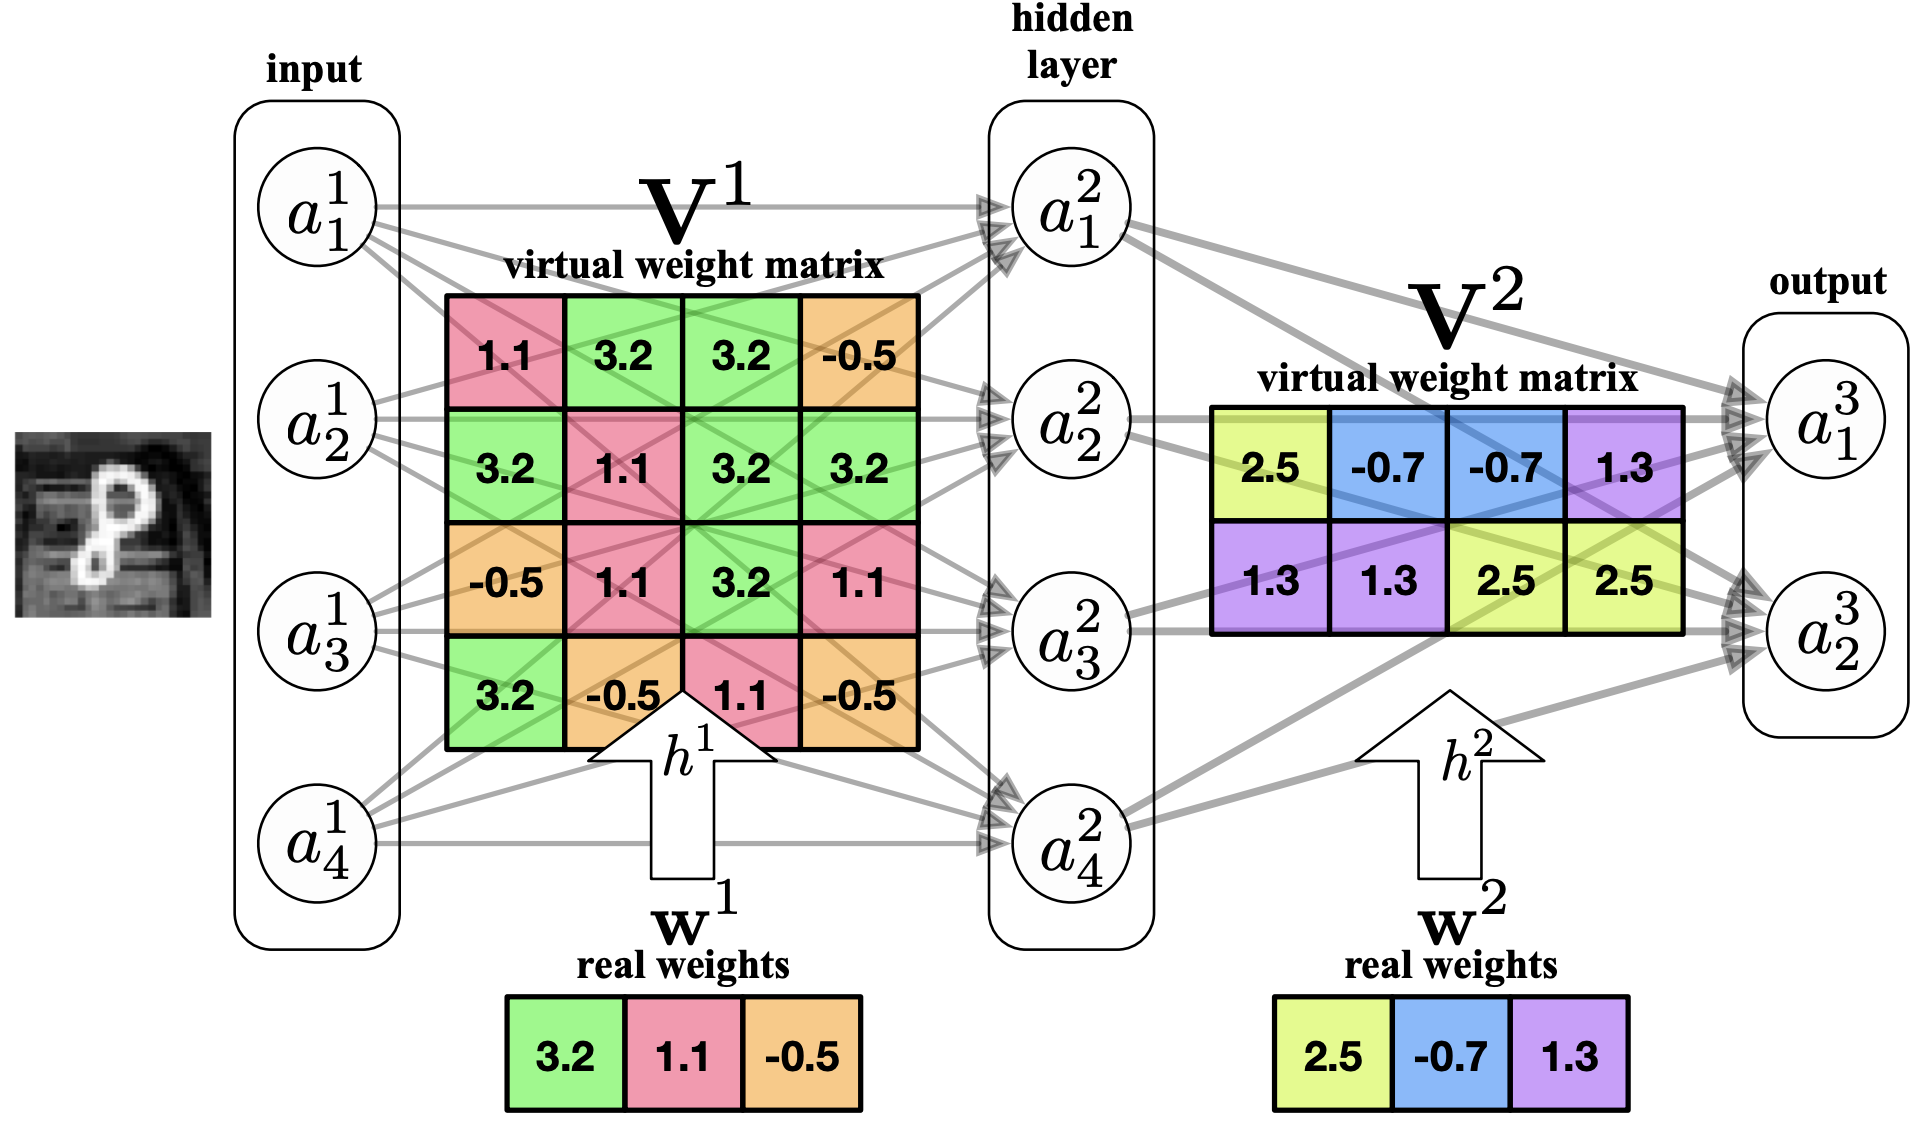
\includegraphics[width=0.7\textwidth]{images/hashednet.png}
    \caption{HashedNet illustration \cite{HashedNet}. This can be seen as random weight sharing}
    \label{fig:hashed_net}
\end{figure}
\end{frame}


\subsection{Multi-hashing}
\begin{frame}{Multi-hashing}
\begin{itemize}
    \pause\item One can obtain greater flexibility with \textit{multi-hashing}
    \pause\item Create $m$ variables buckets $\nu_1, ..., \nu_m$ and $m$ hashing functions $h_1, ..., h_m$
    \pause\item Each $h_k$ maps parameter's index $i$ into its bucket's index $\nu_k[h_k(i)]$
    \pause\item To obtain the value for $\theta_i$, compute:
    \begin{equation}\label{eq:multi-hashing}
        \theta_i = \sum_{k=1}^m \nu_k[h_k(i)]
    \end{equation}
    \pause\item Instead of summation one can use other reducing functions, like product, max, min, etc.
\end{itemize}
\end{frame}


\begin{frame}{Structured Multi-Hashing}
\begin{itemize}
    \pause\item Traditional multi-hashing lacks memory locality which makes slows things down
    \pause\item \cite{Structured_multi_hashing} solves the problem with a special hashing function
    \pause\item First, they reshape parameters into matrix $M$
    \begin{figure}
        \centering
        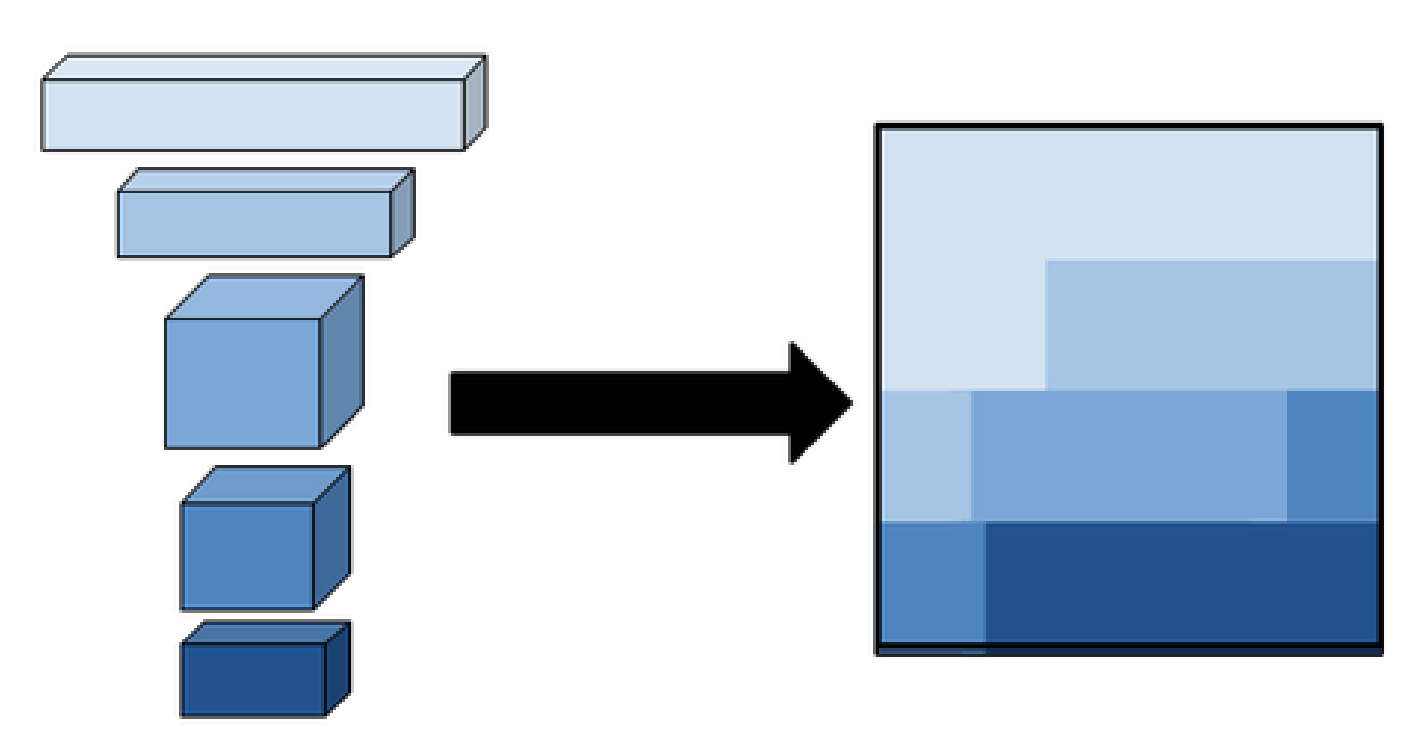
\includegraphics[width=0.5\textwidth]{images/structured-multi-hashing-reshaping.png}
        \caption{Structred Multi-Hashing parameters reshaping}
        \label{fig:smh-reshaping}
    \end{figure}
    \pause\item Then they factorize this matrix into low-rank product $M = UV$
    \pause\item Now $\theta_i$ can be seen as a multi-hashing reduction:
    \begin{equation}
        \theta_i = U_{(s)}^\top V^{(t)} = \sum_{k=1}^m U_{(s),k} V^{(t)}_k
    \end{equation}
\end{itemize}
\end{frame}


\begin{frame}{Structured Multi-Hashing results}
\begin{figure}
\begin{subfigure}{0.47\textwidth}
    \centering
    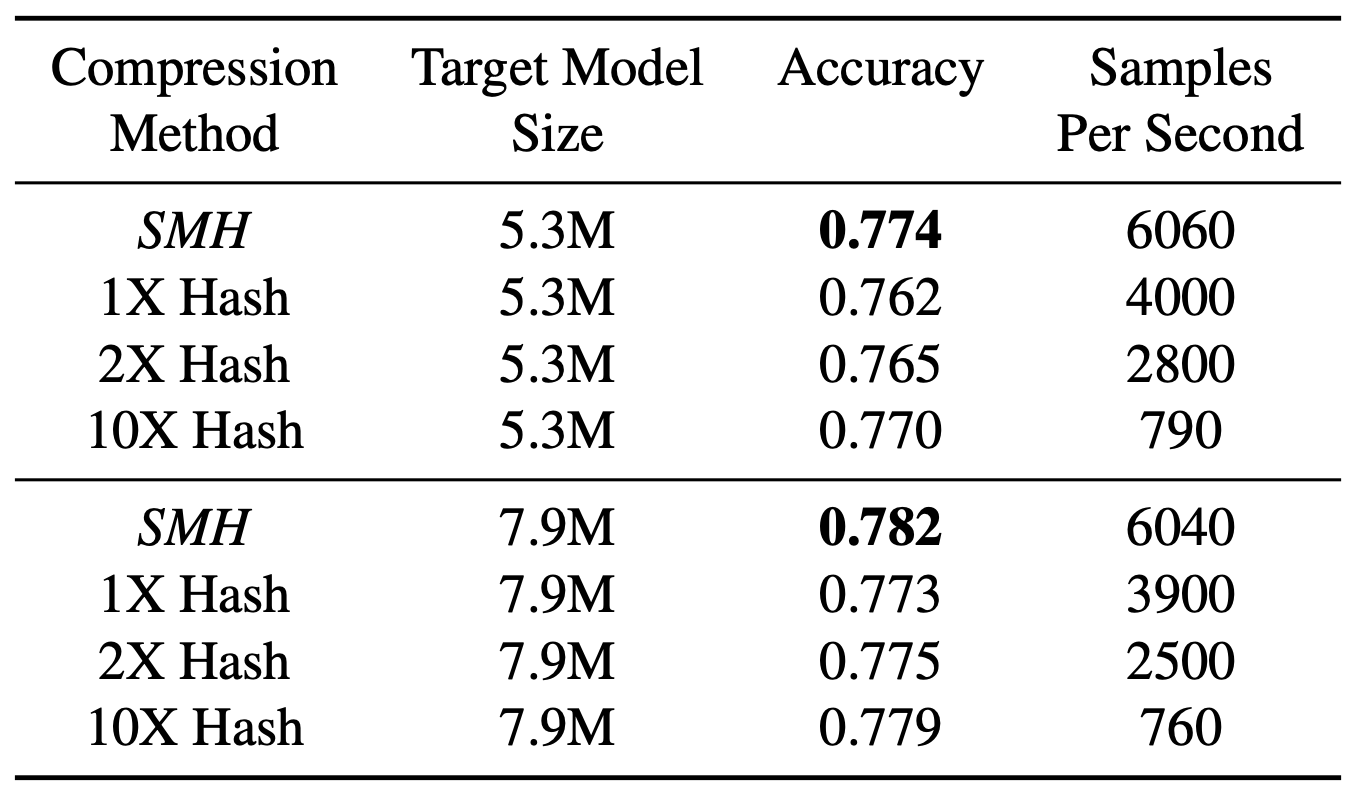
\includegraphics[width=\linewidth]{images/smh-results.png}
\end{subfigure}
\begin{subfigure}{0.47\textwidth}
    \centering
    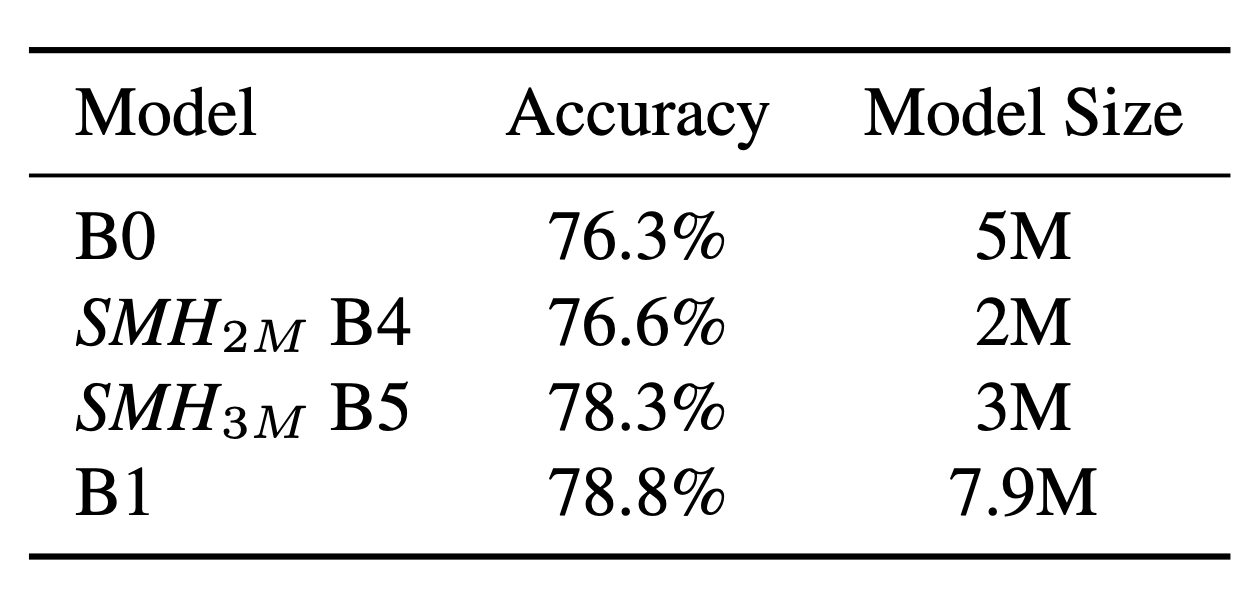
\includegraphics[width=\linewidth]{images/smh-results-extreme-compression.png}
\end{subfigure}
\caption{SMH works much faster and obtains better results for EfficientNet-B2 on Imagenet. It also performs well under extreme compression (up to 10$\times$) for large datasets}
\label{fig:smh-results}
\end{figure}
\end{frame}


\section{Low-rank decomposition}
% \begin{frame}
%     Low-rank decomposition
% \end{frame}

\begin{frame}{Low-rank decomposition}
    \begin{itemize}
        \pause\item Low-rank decomposition usually represents weight tensors as a product of low-rank matrices $W = UV$
        \pause\item This can be done during training or after training
        \pause\item \cite{Low_rank_and_sparse_decomposition} represents it as $W \approx L + S$, where $L$ is low-rank and $S$ is sparse
        \pause\item TTD \cite{TTD} ``tensorizes'' weights and biases by reshaping them into $d$-dimensional tensors and applies \textit{tensor train decomposition}:
        \begin{equation}
        \mathcal{A}\left(j_{1}, \ldots, j_{d}\right)=\boldsymbol{G}_{1}\left[j_{1}\right] \boldsymbol{G}_{2}\left[j_{2}\right] \cdots \boldsymbol{G}_{d}\left[j_{d}\right]
        \end{equation}
        i.e. each element in tensor $\mathcal{A}$ is computed as a product of small matrices
    \end{itemize}
\end{frame}

\section{Quantization}
\begin{frame}
    Quantization
\end{frame}

\begin{frame}{Quantization}
    \begin{itemize}
        \item\pause Quantization converts model weights (and sometimes activations) to a lower precision
        \begin{itemize}
            \item\pause One can train a low-precision model from scratch
            \item\pause But a more practical approach is to quantize a model after training (\textit{post-time quantization})
        \end{itemize}
        \item\pause Practically interesting precisions are fp16, int8
        \item\pause Theoretically interesting precisions are fp16, int8, int4, ternary, binary
    \end{itemize}
\end{frame}


\begin{frame}{Quantization}
    \begin{itemize}
        \pause\item Any quantizers is defined by scale, shift and precision:
        \begin{equation}
            Q_p(x, \gamma, \beta) = \operatorname{round}_p\left( \frac{x}{\gamma} + \beta \right) 
        \end{equation}
        \begin{itemize}
            \item\pause precision $p$ defines the range for a value to be rounded to, i.e. for int8 it is $[0, 1, ..., 255]$
            \item\pause parameters $\gamma$ and $\beta$ normalizes the variable to the required range
        \end{itemize}
        \pause\item Quantizers use equal distances between quantized values since the common hardware is not supposed to work with non-standard non-linear quantization (i.e. different from floats)
        \pause\item Usually, precision $p$ is defined by your needs and your hands are tied in changing it
        \pause\item So the main research question is how to find the best $\gamma$ and $\beta$ for your data.
        % \begin{equation}
        %     Q(x, \text { scale, zero_point })=\operatorname{round}\left(\frac{x}{\text { scale }}+\text { zero_point }\right)
        % \end{equation}
    \end{itemize}
\end{frame}

\begin{frame}{Outlier Channel Splitting (OCS)}
    \begin{itemize}
        \item\pause Usually, people select $\beta,\gamma$ s.t. KL distance between the quantized values and original values is minimal (for histograms)
        \item\pause But OCS\cite{OCS} notices that it makes tails be poorly covered by the quantized distribution
        \item\pause Previously, people just clipped them away
        \item\pause Authors remove these outliers (channels with large-magnitude weights) by duplicating them and dividing by 0.5
        \item\pause This does not change predictions and has negligible overhead
    \end{itemize}
    
    \begin{figure}
        \centering
        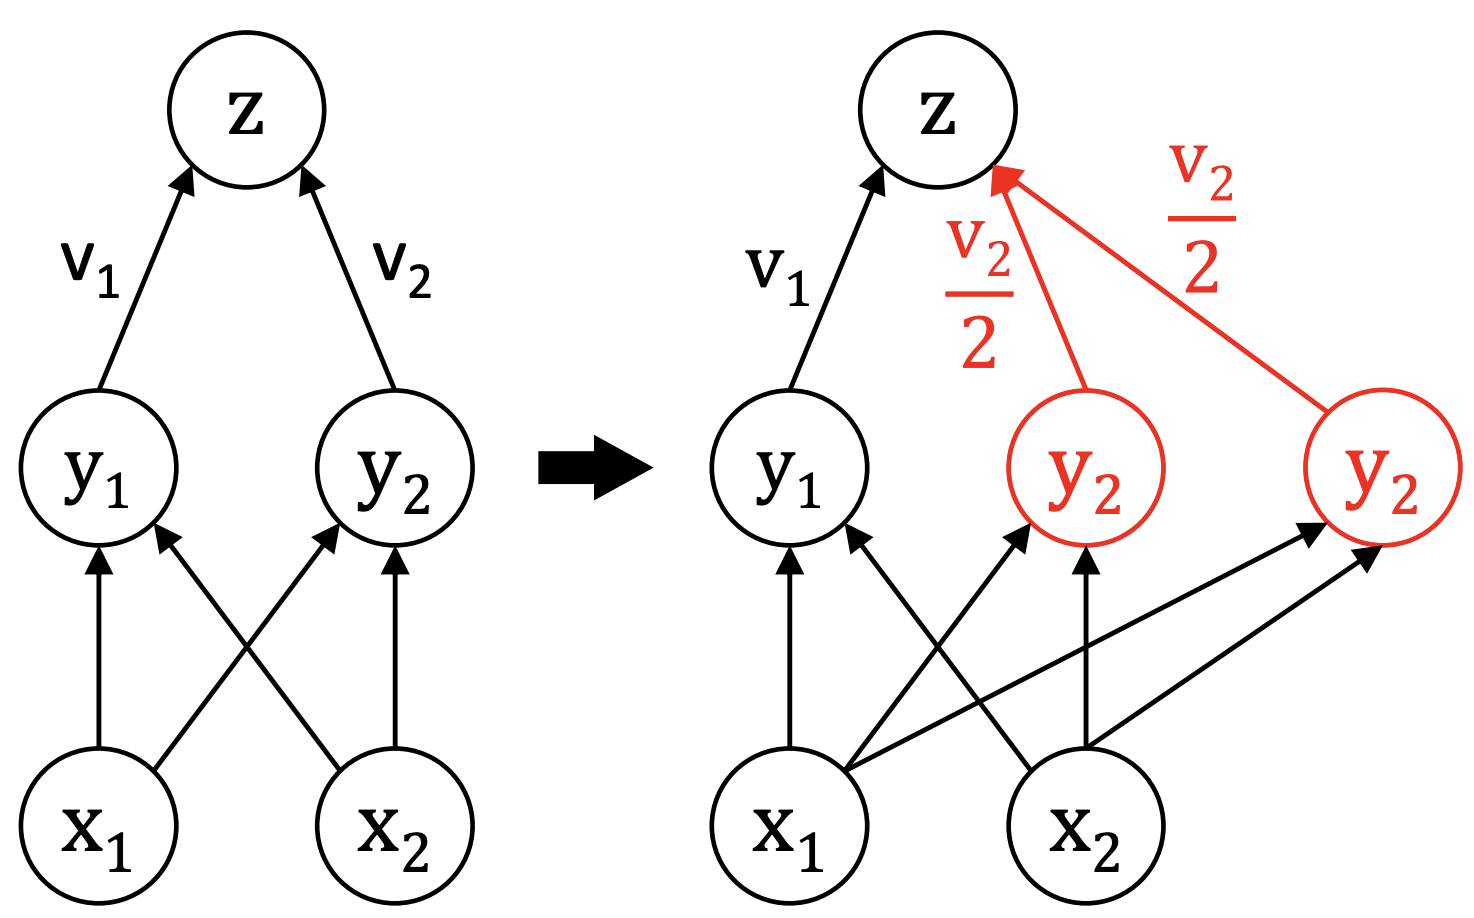
\includegraphics[width=0.4\textwidth]{images/ocs-diag.png}
        % \caption{Caption}
        % \label{fig:my_label}
    \end{figure}
\end{frame}

\begin{frame}{OCS results}
    \begin{figure}
        \centering
        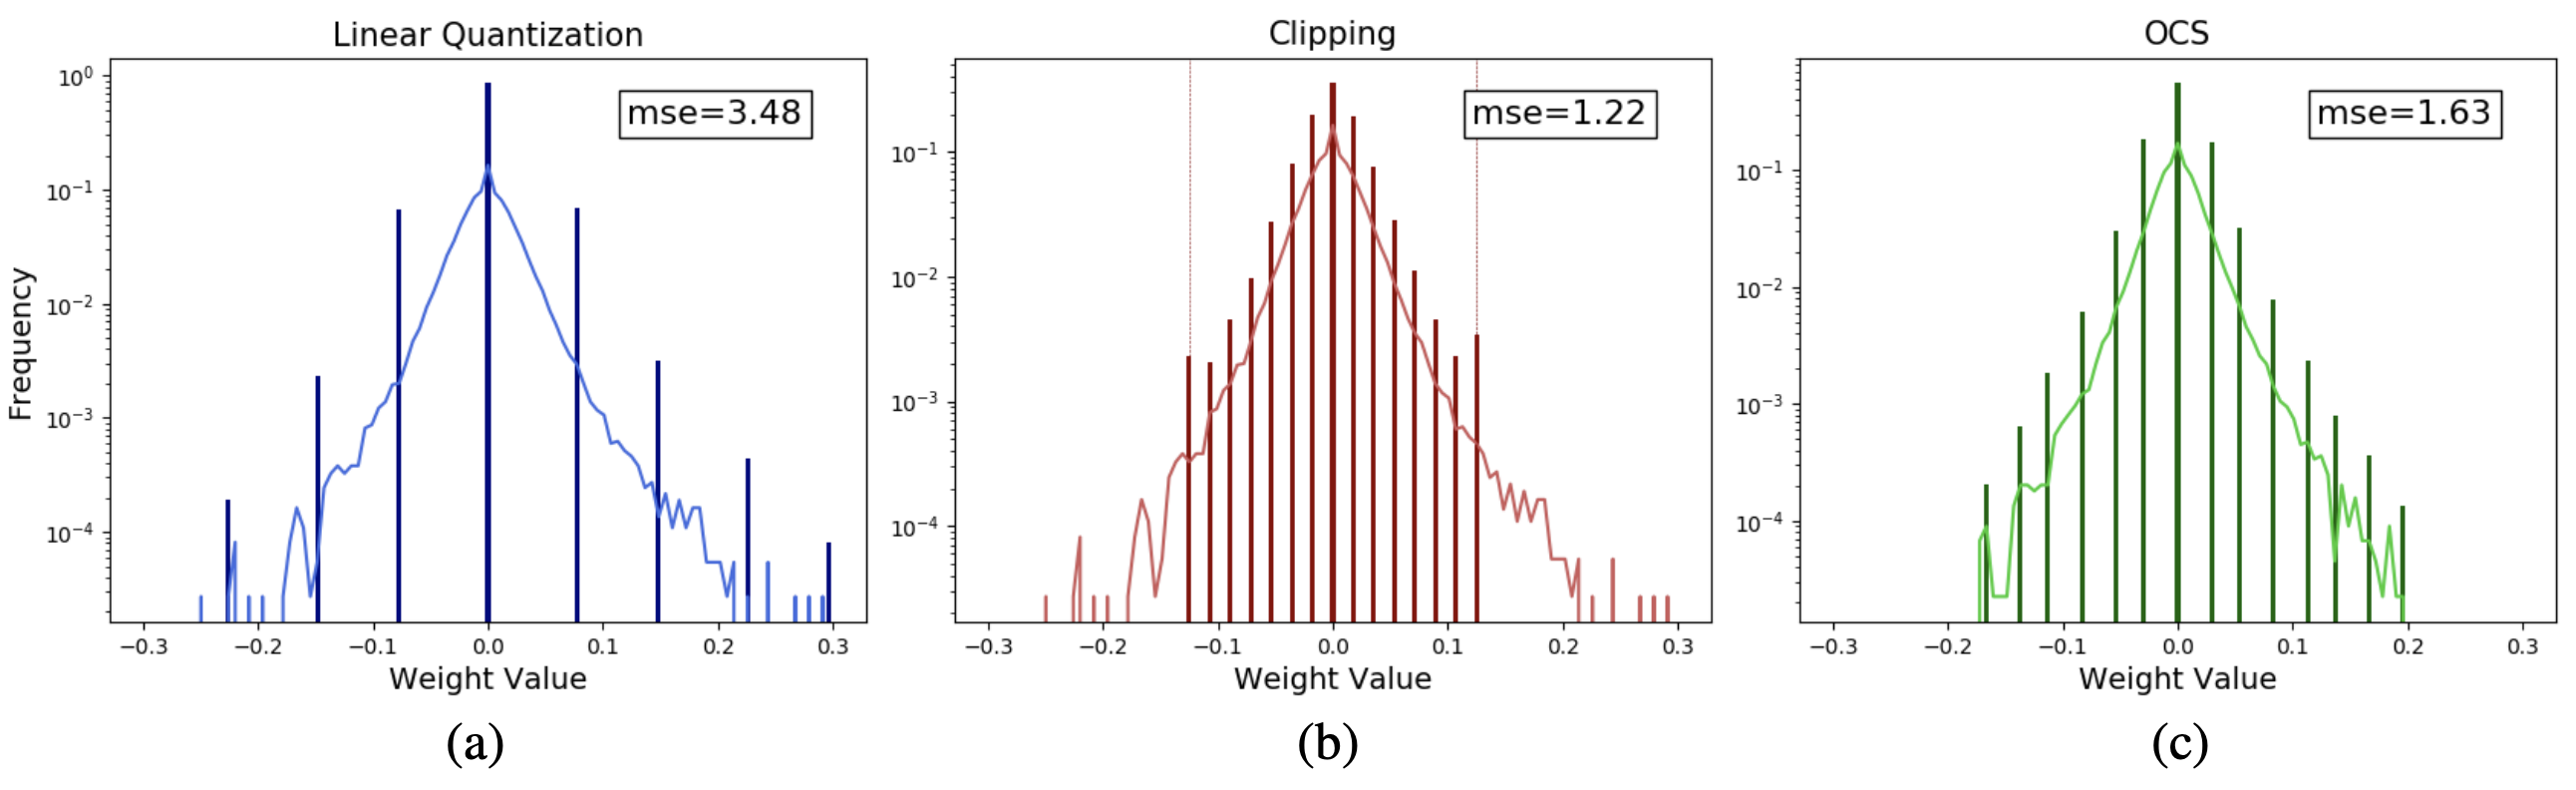
\includegraphics[width=\textwidth]{images/ocs-hists.png}
        % \caption{Caption}
        % \label{fig:my_label}
    \end{figure}
\end{frame}

\section{Other techniques}
\begin{frame}{Knowledge distillation}
    \begin{itemize}
        \item\pause Knowledge distillation distills a big teacher model $M_\phi$ into a small student $f_\theta$
        \item\pause One can use logits instead of one-hot labels since logits carry uncertainty information
        \item\pause Can be done without data \cite{Data_free_adv_knowledge_distillation}: train the student to produce similar outputs on samples from the generator which tries to fool him.
    \end{itemize}
\end{frame}

\begin{frame}{Architectural tricks}
    \pause
    One of the best-performing tricks to compress a model is designing compressed architectures manually:
    \begin{itemize}
        \item\pause Depthwise-separable convolutions
        \item\pause Groupwise convolutions
        \item\pause Conv+Bilinear instead of ConvTranspose
        \item\pause Conv$\to$ReLU$\to$MaxPool$\to$BN instead of Conv$\to$BN$\to$ReLU$\to$MaxPool
        \item\pause BatchNorm fusion: fuse batchnorm computation into the succeeding layer
        \item\pause Early-exit: Resnets with dynamic depths that can classify easier examples earlier \cite{Dynamic_depth}
    \end{itemize}
\end{frame}

\section{Conclusion}
\begin{frame}
    \begin{itemize}
        \item\pause Compression models is important from both practical and theoretical perspective
        \item\pause Most of the methods are interesting, but not quite practical
        \item\pause The most practical methods are quantization and ``architectural tricks''
    \end{itemize}
\end{frame}

\end{document}
